%%%%%%%%%%%%%%%%%%%%%%%%%%%%%%%%%%%%%%%%%%%%%%%%%%%%%%%%%%%%%%%%%%%%%%%%
%                                                                      %
%     File: Thesis_Model_Improvements.tex                              %
%     Tex Master: Thesis.tex                                           %
%                                                                      %
%     Author: João C. Godinho                                          %
%     Last modified : Apr 2018                                         %
%                                                                      %
%%%%%%%%%%%%%%%%%%%%%%%%%%%%%%%%%%%%%%%%%%%%%%%%%%%%%%%%%%%%%%%%%%%%%%%%

\chapter{Model Improvements}
\label{chapter:model_improvements}

Having a solid baseline model for our malware detection task together with how laboratory \textit{vs.}\ real-world scenarios change the model outcome, we now take this chapter to present the improvements made in order to obtain a more robust model to detect malware.
We start by describing our first improvement, applying a multi layer model to extract more information regarding a sample.
We then take this enhanced model and increase the number of features to include dynamic content and how it impacted the model's results.

%%%%%%%%%%%%%%%%%%%%%%%%%%%%%%%%%%%%%%%%%%%%%%%%%%%%%%%%%%%%%%%%%%%%%%%%
\section{Multi Layer Model}
\label{section:improvements_multi_layer}

On the previous chapter we ended up with a simple \gls{lr} model $\LR$ that given a set of static imports from a sample, would give the probability of it being malware.
Although that was the end purpose of our work, it does not give any deeper understanding of the sample, other than being or not malware.
With that in mind, we propose a new model that not only provides the probability of a sample being malware, but also the probability of being from a specific malware type.

This new model $\mathcal{E}$ comprises a simple ensemble stacking approach, which instead of using a single \gls{lr} classifier, multiple ones are used, layered into two steps.

The first step (layer $\mathcal{E}_{\mathcal{L}_{0}}$) is composed of $n$ \gls{lr} models, where $n$ is the number of possible classes.
Each model is trained to output the likelihood of sample belonging to one of the $n$ classes, in a \textit{one-vs-all} methodology (\ie\ a sample either belongs to $\mathcal{C}_{n}$ or not), having as input the raw features (\eg\ static imports).

The second step (layer $\mathcal{E}_{\mathcal{L}_{1}}$) is identical to $\mathcal{LR}$, but now takes as features the output of each classifier from the previous layer, outputting the likelihood of a sample being malware.

In summary, as depicted in Figure \ref{fig:dia_multilayer}, we define a 2 layer ensemble stacking with $n$ classifiers on the first layer to a single classifier in the second layer.

\begin{figure}[!htb]
	\centering
	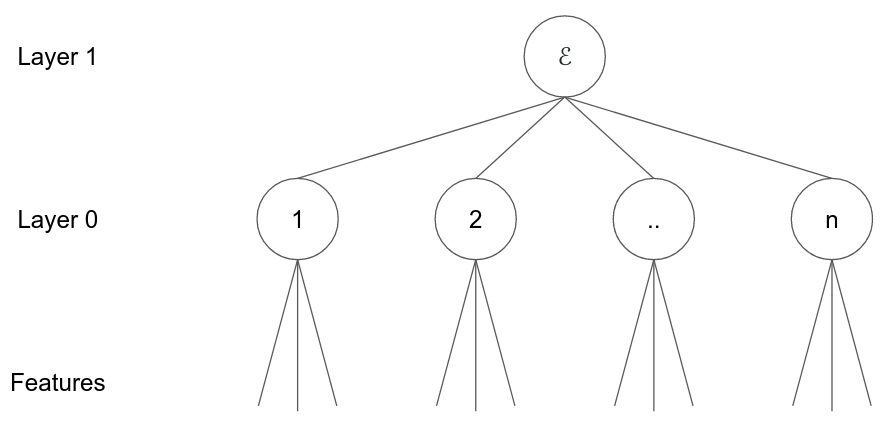
\includegraphics[width=0.8\textwidth]{Figures/dia_multilayer.png}
	\caption{Multi layer model representation.}
	\label{fig:dia_multilayer}
\end{figure}

%%%%%%%%%%%%%%%%%%%%%%%%%%%%%%%%%%%%%%%%%%%%%%%%%%%%%%%%%%%%%%%%%%%%%%%%
\subsection{Malware Classes}

With this new model defined, we now present our approach on selecting the $n$ classes of interest.
This represents another labeling problem, but now instead of having to label between goodware and malware, we have to label the malware as belonging to some subclass.

To choose the malware classes for our datasets, we take into account our description in Chapter \ref{chapter:related_work} regarding propagation methods and malware names based on purpose.
With this in mind, we chose 6 malware classes: \textit{virus}, \textit{trojan}, \textit{worm}, \textit{ransom}, \textit{spyware} and \textit{other}.
The first three classes, \textit{virus}, \textit{trojan} and \textit{worm}, were chosen from the propagation methods, whereas \textit{ransom} and \textit{spyware}
where chosen due to their popularity in recent years. The last class, \textit{other}, serves for any malware that does not fit the previous five.

As mentioned in Chapter \ref{chapter:related_work}, there is no agreed upon naming convention for malware, which translates into different names for the same malware sample.
To minimize this problem, we referenced a tool by Sebastián, M. et al.~\cite{sebastian2016avclass}, AVClass, which was built to normalize a malware sample name into the most likely family, using the names provided by VirusTotal~\cite{tool:virustotal}.

We took advantage of this tool and modified it such that instead of providing a family name, it would provide one (or more) of the 6 previously defined classes.
Specifically, we changed it in a way that given a set of malware names, the output would be a distribution over the 6 malware classes.

To calculate each class weight we apply the following formula
\begin{eqnarray*}
	\mathcal{W}_c = \dfrac{f_c}{\sum\limits_{c}f_c}
\end{eqnarray*}

where $f_c$ is the frequency for the class $c$ and $\sum_{c}f_c$ is the number of times all classes appear.
For example, if a given set of names contain the name \textit{trojan} 3 times and the name \textit{virus} one time, then the weights would be
\begin{eqnarray*}
	\mathcal{W}_{trojan}=\dfrac{3}{4}=0.75,~\mathcal{W}_{virus}=\dfrac{1}{4}=0.25,~ \mathcal{W}_{c}=0, c \in \{worm, spyware, other, ransom\}
\end{eqnarray*}

\medskip

Having these malware classes defined for our multi layer model, we also added the \textit{goodware} class for samples that are not malware.
Doing so gives us 7 possible classes, 6 of which are malware only.
It is worth mentioning that if a sample belongs to the \textit{goodware} class, it cannot belong to any other, likewise if it belongs to any malware class, it cannot belong to the \textit{goodware} class.

In sum, we added a layer of labeling to our dataset, where a sample can either belong to the \textit{goodware} class, or to a set of the other 6 malware classes.
This concludes our first improvement to our model, what follows are our improvements regarding features.

%%%%%%%%%%%%%%%%%%%%%%%%%%%%%%%%%%%%%%%%%%%%%%%%%%%%%%%%%%%%%%%%%%%%%%%%
\section{Dynamic Features}
\label{section:improvements_dynamic_features}

%%%%%%%%%%%%%%%%%%%%%%%%%%%%%%%%%%%%%%%%%%%%%%%%%%%%%%%%%%%%%%%%%%%%%%%%
\section{Improved Model Results}
\label{section:improvements_results}